\cchapter{مقدمه}
\par
امنیت در رای‌گیری همواره یک مسئله‌ی پیچیده بوده است که نیازمند یک فرد قابل اعتماد برای برگزاری و یک پروتکل امن برای جلوگیری از تقلب یا اشتباه در فرایند آن است. سیستم‌های رای‌گیری الکترونیک 

از سال ۱۹۶۰ وجود داشتند و اولین استفاده‌ بزرگ از آن‌ها در چند ایالت آمریکا در سال ۱۹۶۴ برای انتخابات ریاست جمهوری بود. رای‌گیری الکترونیک به‌سادگی می‌تواند هزینه برگزاری انتخابات را از طریق سادگی شمارش کاهش دهد. 

\section{فرایند رای‌گیری ایده‌آل}

شروط فرایند رای‌گیری ایده‌آل عبارت‌ است از:
\begin{itemize}
	\item 
	هر فرد واجد شرایط دقیقا یک بار بتواند رای دهد.
	\item 
	هیچ کسی نتواند به جای فرد دیگری رای دهد.
	\item 
  	هیچ فردی مجبور به رای دادن نشود.
  	\item 
  	هیچ فردی مجبور به رای دادن به کاندیدای خاصی نشود.
  	\item 
  	از شمارش هر رای اطمینان حاصل شود.
  	\item 
    نتیجه‌ی آرا ناشناس  باقی بماند. 
  	\item 
  	بسته به نیاز بتوان نتایج لحظه‌ای انتخابات را (بدون آسیب به شرط‌های قبلی) دید.
\end{itemize}

\section{سیستم‌های رای‌گیری سنتی}
\par
در رای‌گیری غیر الکترونیکی معمولا فرایند به شکل زیر است:
\\
فرد برای رای‌دادن به یکی از حوزه‌های رای‌گیری مراجعه کرده و با ارائه‌ی مدارک شناسایی خود یک برگه‌ی رای دریافت می‌کند. برگه رای دارای دو بخش است: قسمتی که برای ردیابی با اطلاعات شخصی فرد پر می‌شود و یک قسمت بی‌نام که فرد کاندیدای مورد نظر خود را در آن ثبت کرده و در یک صندوق می‌اندازد. 
\\
با بررسی مدارک شناسایی، شرط دوم فرایند رای‌گیری ایده‌آل تایید شده و با ثبت شدن اطلاعات فرد به عنوان یک رای‌دهنده از رای دادن دوباره‌ی او جلوگیری می‌شود. امنیت شخصی افراد در حوزه توسط برگزارکننده‌ی انتخابات تامین می‌شود و با وجود گزینه‌ی «رای سفید» فردی مجبور به رای دادن و یا رای دادن به یک کاندیدای خاص نمی‌شود. 
\\
با وجود یک صندوق برای چندین رای و نبودن هیچ نشانه‌ی شناسایی در آرا، هیچ راهی برای فهمیدن رای یک فرد خاص - حتی اگر برگه‌های رای به دست رقیب بیفتد - وجود ندارد. 
\\
احزار هویت و شمارش رای‌ها به عهده‌ی برگزارکننده‌ی انتخابات است و تنها از طریق یک شخص ثالث برای باز‌شماری آرا می‌توان از اجرای درست آن‌ها اطمینان حاصل کرد.
\\
با توجه به هزینه‌ی زیاد شمارش در انتخابات‌های بزرگ راهی برای اعلام لحظه‌ا‌ی نتایج با هزینه‌ی معقول وجود ندارد.
\\
همانطور که می‌بینیم در روش‌های فعلی انتخابات بسیاری از شرایط مورد نیاز یک انتخابات خوب  با هزینه‌ی نسبتا زیاد فراهم می‌شود. از دیگر مشکلات انتخابات به این روش می‌توان به نیازمندی به یک برگزارکننده‌ی مورد اعتماد اشاره کرد. باید به برگزارکننده اعتماد شود تا: 
\begin{enumerate}
	\item 
	امنیت حوزه‌ی انتخابات را تامین کند.
	\item 
	افراد را به درستی احراز هویت کند.
	\item 
	همه‌ی رای‌ها را بشمارد.
	\item 
	تغییری در رای‌ها ندهد.
	
\end{enumerate}
 

\section{مشکلات و چالش‌های رای‌گیری الکترونیک}
\par
دو مسئله‌ی اساسی در یک سیستم رای‌گیری امنیت و حریم خصوصی است. مخالفین رای‌گیری الکترونیک از کم هزینه بودن تقلب و تغییر رای‌های ثبت شده در انتخابات الکترونیکی می‌گویند و رد کاغذی در یک انتخابات را یک فاکتور مهم برای امنیت آن می‌دانند. هزینه تغییر میلیون‌ها رای در یک سیستم کامپیوتری بسیار پایین‌تر از تولید چند میلیون رای کاغذی تقلبی برای تغییر نتیجه‌ی یک انتخابات است.
\\
بزرگترین مسئله در به‌کارگیری رای‌گیری الکترونیک مسئله‌ی اعتماد به یک سیستم‌ کامپیوتری است. از نظر بسیاری از رای‌دهندگان رای دادن با کامپیوتر شخصی می‌تواند ریسک تغییر رای تا رسیدن آن به سرور‌های رای‌گیری ایجاد کند. از طرف دیگر عدم امکان بررسی و تایید انسانی عملیات کامپیوتر، حس امنیت کمتری القا می‌کند.
\par
مسئله‌ی دیگر پرهزینه بودن ساخت زیرساخت‌های رای‌گیری الکترونیک و خطر پیدایش مشکلات امنیتی در هر سیستم کامپیوتری - چه از نظر نرم‌افزار و چه سخت‌افزار - است. این مشکل باعث شده تعدادی از کشور‌ها از جمله هلند، ایرلند و آلمان فرایند ایجاد زیرساخت لازم را شروع کرده و در ادامه این فرایند را ملقی کنند. دلیل اصلی اعلام شده برای این مسائل‌ قابل اتکا نبودن سیستم‌های رای‌گیری الکترونیکی اعلام شده است. 
\\
برای مثال یک تحقیق معروف از دانشگاه‌ \lr{NYU} در سال ۲۰۱۵ 
\LTRfootnote{https://www.brennancenter.org/publication/americas-voting-machines-risk}
توضیح داد که ماشین‌های رای‌گیری الکترونیکی که در ۴۳ ایالت آمریکا استفاده می‌شوند در سال ۲۰۱۶ به دهمین سال استفاده شدن می‌رسند و به دلیل نداشتن بودجه‌ی کافی برای تعمیرات و بروزرسانی، در معرض خطر کرش
\LTRfootnote{crash}
 کردن هستند که می‌تواند باعث کندی فرایند و حتی گاها از دست رفتن را‌ی‌های مردم شود. علاوه بر این، قدیمی بودن دستگاه‌ها می‌تواند ریسک‌های امنیتی ایحاد کند. 

\par
یک مشکل دیگر در پیاده‌سازی‌های بسیاری از رای‌گیری الکترونیک، نیاز به اینترنت و توانایی استفاده از کامپیوتر است. این مسئله می‌تواند دسترسی بسیاری از افرادی واجد شرایط را - به دلیل نقص جسمی و یا عدم توانایی کار با کامپیوتر - محدود کند. در سیستم‌های فعلی که مبتنی بر حوزه‌های رای‌گیری هستند می‌توانند با کمک انسانی در خود حوزه تا حدی این مشکلات را رفع کنند. 
\par
مشکلات مطرح‌ شده موانع بزرگی برای فراگیری سیستم‌های رای‌گیری کاملا الکترونیکی برای انتخابات‌های مهم و بزرگ هستند که یک سیستم رای‌گیری مناسب باید آن‌ها را تا جای ممکن رفع کند. 

\section{انگیزه و هدف}
هدف این تحقیق، طراجی یک سیستم رای‌گیری الکترونیک است که شرایط رای‌گیری ایده‌آل را تا جای ممکن بدون نیاز به اعتماد به شخص ثالث ایفا کند. با فراگیری تکنولوژی بلاک‌چین برای ایچاد سیستم‌های توزیع شده بدون نیاز به اعتماد (برای مثال بیت‌کوین به عنوان یک‌ ارز دیجیتال بدون نیاز به اعتماد)، پلتفرم‌هایی برای رای‌گیری الکترونیک ایجاد شدند که امنیت شمارش آرا را با عمومی ساختن فرایند رای‌گیری تامین می‌کردند. 
\\
با وجودی که راه‌حل ارائه شده‌ی این سیستم‌ها مسئله‌ی اطمینان از شمارش رای‌ها را حل می‌کرد، مسئله‌ی حریم شخصی در این روش‌ها حل نشده است و انتخابات‌های برگزار شده با این سیستم‌ها امنتیت کمتری در قبال ناشناس ماندن رای‌ها ارائه می‌کنند. 
\\
برای مثال حالتی را فرض کنید که یک رای‌دهنده تهدید می‌شود که باید به یک کاندیدای خاص رای بدهد، در سیستم‌های سنتی رای‌گیری به دلیل بی‌نام بودن برگه‌های رای بعد از اتمام فرایند رای‌گیری راهی برای اطمینان حاصل کردن از نتیجه‌ی رای فرد نیست. از طرفی به دلیل امنیت حوزه‌های رای‌گیری راهی برای اطمینان از نتیجه‌ی رای یک نفر در حین فرایند رای‌گیری هم نیست. پس راهی برای محبور کردن یک نفر که به یک کاندیدای خاص رای بدهد وجود ندارد. اما در سیستم‌های مبتنی بر بلاک‌چین هر رای داده شده به امضای الکترونیکی فرد امضا شده است و این موضوع می‌تواند با عمومی شدن بلاک‌چین بعد از رای‌گیری باعث لو رفتن نتیجه‌ی رای آن فرد شود.
\\
این مشکلات مانع بزرگی برای استفاده‌ی فراگیر این سیستم‌ها خواهد بود. هدف ما در این تحقیق ارائه امنیت و هزینه‌ی کم ناشی از استفاده از این روش‌های رای‌گیری، بدون ایجاد ریسک‌های جدید در حریم خصوصی رای‌دهندگان است. 
\par
نتیجه‌ی این تحقیق یک سیستم‌ رای‌گیری الکترونیک است که قیاس با سیستم‌های سنتی انتخابات هزینه‌ها را کاهش خواهد داد. در عین حال کمترین تغییر برای رای‌دهندگان خواهد داشت که باعث افزایش دسترس‌پذیری این سیستم خواهد شد. همچنین تمامی آرا رای‌دهندگان در قبال یک مهاجم خارجی و حتی خود برگزار کننده‌ی انتخابات ناشناس خواهند ماند. 
\\
از طرفی این سیستم یک رد الکترونیک غیرقابل انکار از تمام ارا، در قبال یک بلاک‌چین، ارائه ‌خواهد کرد که توانایی اثبات درستی شمارش را برای شخص ثالث بدون ایجاد خطری برای ناشناسی رای‌ها خواهد داد. 
\\
تمامی این قابلیت‌ها بدون نیاز اعتماد به برگزارکننده‌ی انتخابات خواهد بود و هرگونه تخطی از پروتکل ارائه شده توسط حوزه‌های رای‌گیری قابل ردیابی از طریق اطلاعات ثبت شده در بلاک‌چین خواهد بود.








\cchapter{تعریف مفاهیم}
در این بخش به معرفی بعضی مفاهیم پایه برای این تحقیق می‌پردازیم. در ابتدا با مفاهیم بلاک‌چین و انواع و کاربرد‌های آن آشنا می‌شویم و در ادامه به بررسی اثبات‌های بی‌دانش می‌پردازیم. این دو تکنولوژی ابزارهای تئوری لازم برای ساخت سیستم رای‌گیری امن خواهند بود.
\section{بلاک‌چین}
بلاک‌چین ساختمان‌داده‌ایست که به مانند لینک‌‌لیست
\LTRfootnote{Linked list}
از بلوک‌‌های متوالی تشکیل شده ولی در بلاک‌چین هر بلوک هش
\LTRfootnote{Hash}
عنصر قبلی خود را نیز نگه‌می‌دارد. هدف از این کار ساخت یک ساختار داده‌ی صرفا افزایشی 
\LTRfootnote{Append only}
است که در آن‌ بلوک‌های قبلی تغییرناپذیرند. تغییر هر بلوک باعث تغییر بلوک بعدی خواهد شد و این موضوع تشخیص تغییر در بلوک‌های پیشین را بسیار ساده می‌کند.
\section{درخت مرکل}


برای پیاده‌سازی یک بلاک‌چین معمولا از درخت مرکل
 \LTRfootnote{Merkle tree}
 استفاده‌ می‌شود. درخت مرکل یا درخت هش، نوعی درخت دودویی 
 \LTRfootnote{Binary tree}
 است که در آن هر راس هش فرزندان خود را نگه‌داشته و برگ‌ها هش داده‌ی ذخیره‌شده در خودشان را نگه می‌دارند. این روش نگه‌داری اطلاعات باعث می‌شود که درچه‌ی زمانی بررسی وجود یک بلوک داده در بلاک‌چین از 
 \lr{N}
 به 
$ \log N$
 کاهش یابد. به دلیل این نوع ساختار یک درخت مرکل، هر تغییری در درخت باعت تغییر هش در ریشه‌ی آن خواهد شد و به دلیل رندم بودن خروچی یک هش خوب، هش ریشه‌ی درخت مرکل هیچ ویژگی قابل پیشبینیی ندارد.
 
 \begin{figure}[th!]
 	\centering
 	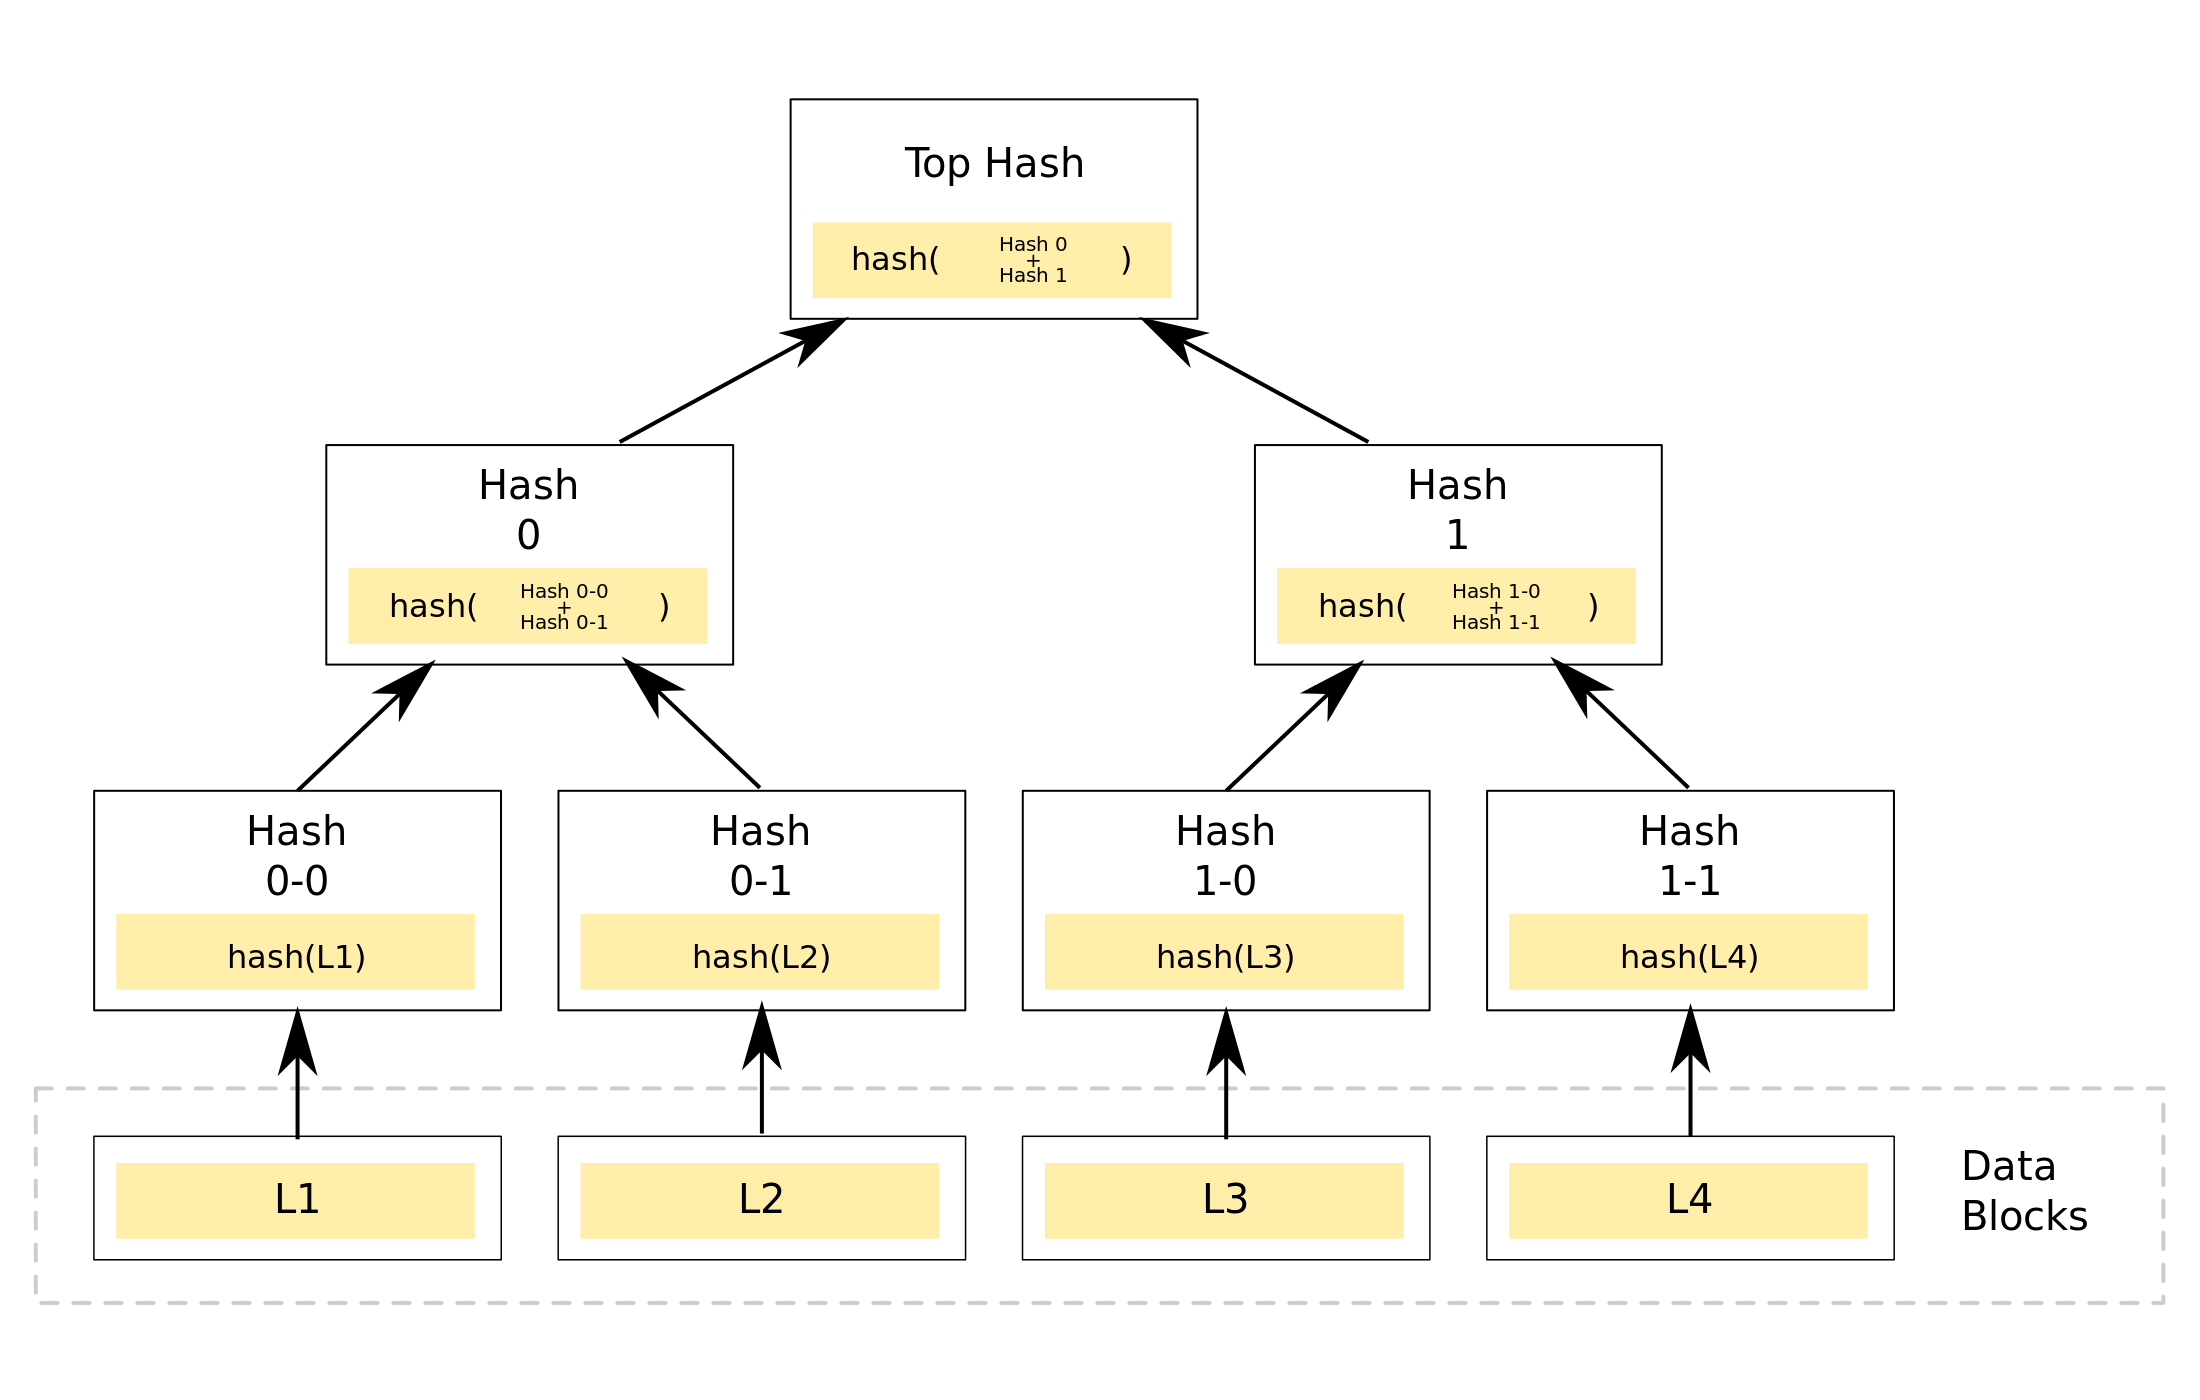
\includegraphics[width=.7\linewidth]{Hash_Tree.png}
 	\caption {یک درخت مرکل}
 	\label{fig:merkle}
 \end{figure}
 
\section{اثبات‌های بی‌دانش}
اثبات‌ بی‌دانش 
\LTRfootnote{Zero knowledge proofs}
روشی است که یک «اثبات‌کننده» می‌تواند یه یک «بررسی‌کننده» نشان دهد که او یک راز - مثلا خروجی یک عملیات کامپیوتری - را می‌داند، بدون این که به بررسی‌کننده هیچ اطلاعات اضافه‌ای، مانند خروجی عملیات، بدهد. به عبارت دیگر اثبات‌های بی‌دانش، صرفا داشتن اطلاعات را اثبات می‌کنند و خود اطلاعات را محفوظ نگه‌ می‌دارند.
\\
یک اثبات بی‌دانش باید ۳ شرط زیر را داشته باشد:
\begin{itemize}
	\item
	کامل‌بودن: اگر گزاره‌ی مورد اثبات صحیح باشد، بررسی‌کننده‌ای که پروتکل را رعایت کند، باید از درستی گزاره مطمئن شود.
	\item 
	درستی: اگر گزاره مورد اثبات غلط باشد، هیچ اثبات‌کننده‌ای نتواند اثباتی ارائه کند که گزاره درست است. 
	\item 
	بی‌دانش: اگر اثبات درست باشد، بررسی کننده هیچ اطلاعاتی فراتر از این که گزاره صحیح است دریافت نکند. به عبارت دیگر 
\end{itemize}
اثبات‌های بی‌دانش، اثبات‌های احتمالاتی هستند و در واقع احتمال کمی وجود دارد که بتوان یک اثبات نادرست ارائه کرد. به بیان دیگر شرط درستی این است که احتمال تولید یک اثبات نادرست بسیار کم باشد. 
\subsection{مثال شهودی}
سناریویی را در نظر می‌گیریم که یک توپ سبز و یک توپ قرمز روی یک میز قرار دارد و آلیس می‌خواهد به باب که کوررنگ سبز و قرمز است ثابت کند که که این دو توپ با هم تفاوت دارند. برای اثبات آلیس چشمش را می‌بندد و باب یا دو توپ را جابجا می‌کند و یا جابجا نمی‌کند. در ادامه آلیس می‌گوید که آیا جای توپ‌ها با هم عوض شده‌اند یا نه. با یک پاسخ درست باب می‌فهمد که آلیس با احتمال ۵۰٪ درست می‌گوید. این فرایند را تا جایی که باب به احتمال دلخواهش برسد ادامه می‌دهند.
\par
یک نکته‌ی مهم در مثال بالا این است که حتی اگر باب این فرایند را ضبط کرده باشد، نمی‌تواند به کس دیگری اثبات کند که آلیس تفاوت این دو توپ را می‌داند چون که راهی برای اثبات این که سوال و جواب از قبل هماهنگ نشده بوده است ندارد. 
\\
این یکی از نیازمندی‌های بی‌دانش بودن اثبات است. اگر در فرایند برای تصمیم‌گیری در تعویض توپ‌ها باب از شیر یا خط کردن یک سکه استفاده می‌کرد، دیگر این اثبات بی‌دانش نبود، چرا که باب می‌توانست با ضبط کردن این فرایند به یک شخص ثالث اثبات کند که آلیس تفاوت این دو توپ را می‌داند. 
\\
برای داشتن شرط بالا یک اثبات بی‌دانش همواره تعامل از سمت بررسی‌کننده نیاز دارد. اما با ریلکس کردن این شرط و استفاده از یک ورودی غیرقابل پیشبینی برای تولید سوال‌های یک اثبات بی‌دانش - مثلا هش ریشه‌ی یک درخت مرکل - می‌توان اثبات‌های بی‌دانش بدون نیاز به تعامل بررسی‌کننده ساخت. 


\subsection{اثبات‌های بی‌دانش بدون تعامل} 
منظور از اثبات بدون تعامل، اثباتی‌ است که در آن نیازی به فرستادن پیامی از سمت بررسی‌کننده به اثبات‌کننده نباشد. با این روش‌ها اثبات‌کننده می‌تواند اثبات را مستقل از بررسی‌کننده بسازد و ارسال کند، در ادامه‌ی این تحقیق اثبات‌های بی‌دانش و بی‌تعامل را 
\textbf{شاهد}
می‌نامیم. در ادامه دو روش تولید یک شاهد بی‌دانش را بررسی می‌کنیم. این روش‌ها می‌توانند برای خروجی هر محاسبات کامپیوتری شاهد ایجاد کنند. 

\subsubsection{ZK-SNARK}
این روش مخفف
\lr{Zero-Knowledge Succinct Non-Interactive Argument of Knowledge}
است. شاهد‌های این روش علاوه بر بی‌دانش بودن ویژگی‌های زیر را دارند:
\begin{itemize}
	\item 
	مختصر
	\LTRfootnote{Succinct}
	: تولید و بررسی شاهد از انجام خود محاسباتی که اثبات می‌شود کوتاه‌تر (معمولا از مرتبه‌ی زمانی $ (\log N) ^ 2$) است. 
	\item
	بی‌تعامل
	\LTRfootnote{Non-Interactive}
	: نیازی به پیامی از بررسی‌کننده برای ایجاد شاهد نیست. 
	\item
	ادعای دانش
	\LTRfootnote{Argument of Knowledge}
	: اثبات ارائه شده در این روش درست 
	\LTRfootnote{Sound}
	است و نمی‌شود بدون داشتن اطلاعات آن را در زمان محدود ساخت.
	
\end{itemize}
 
\begin{figure}[bh]
	\centering
	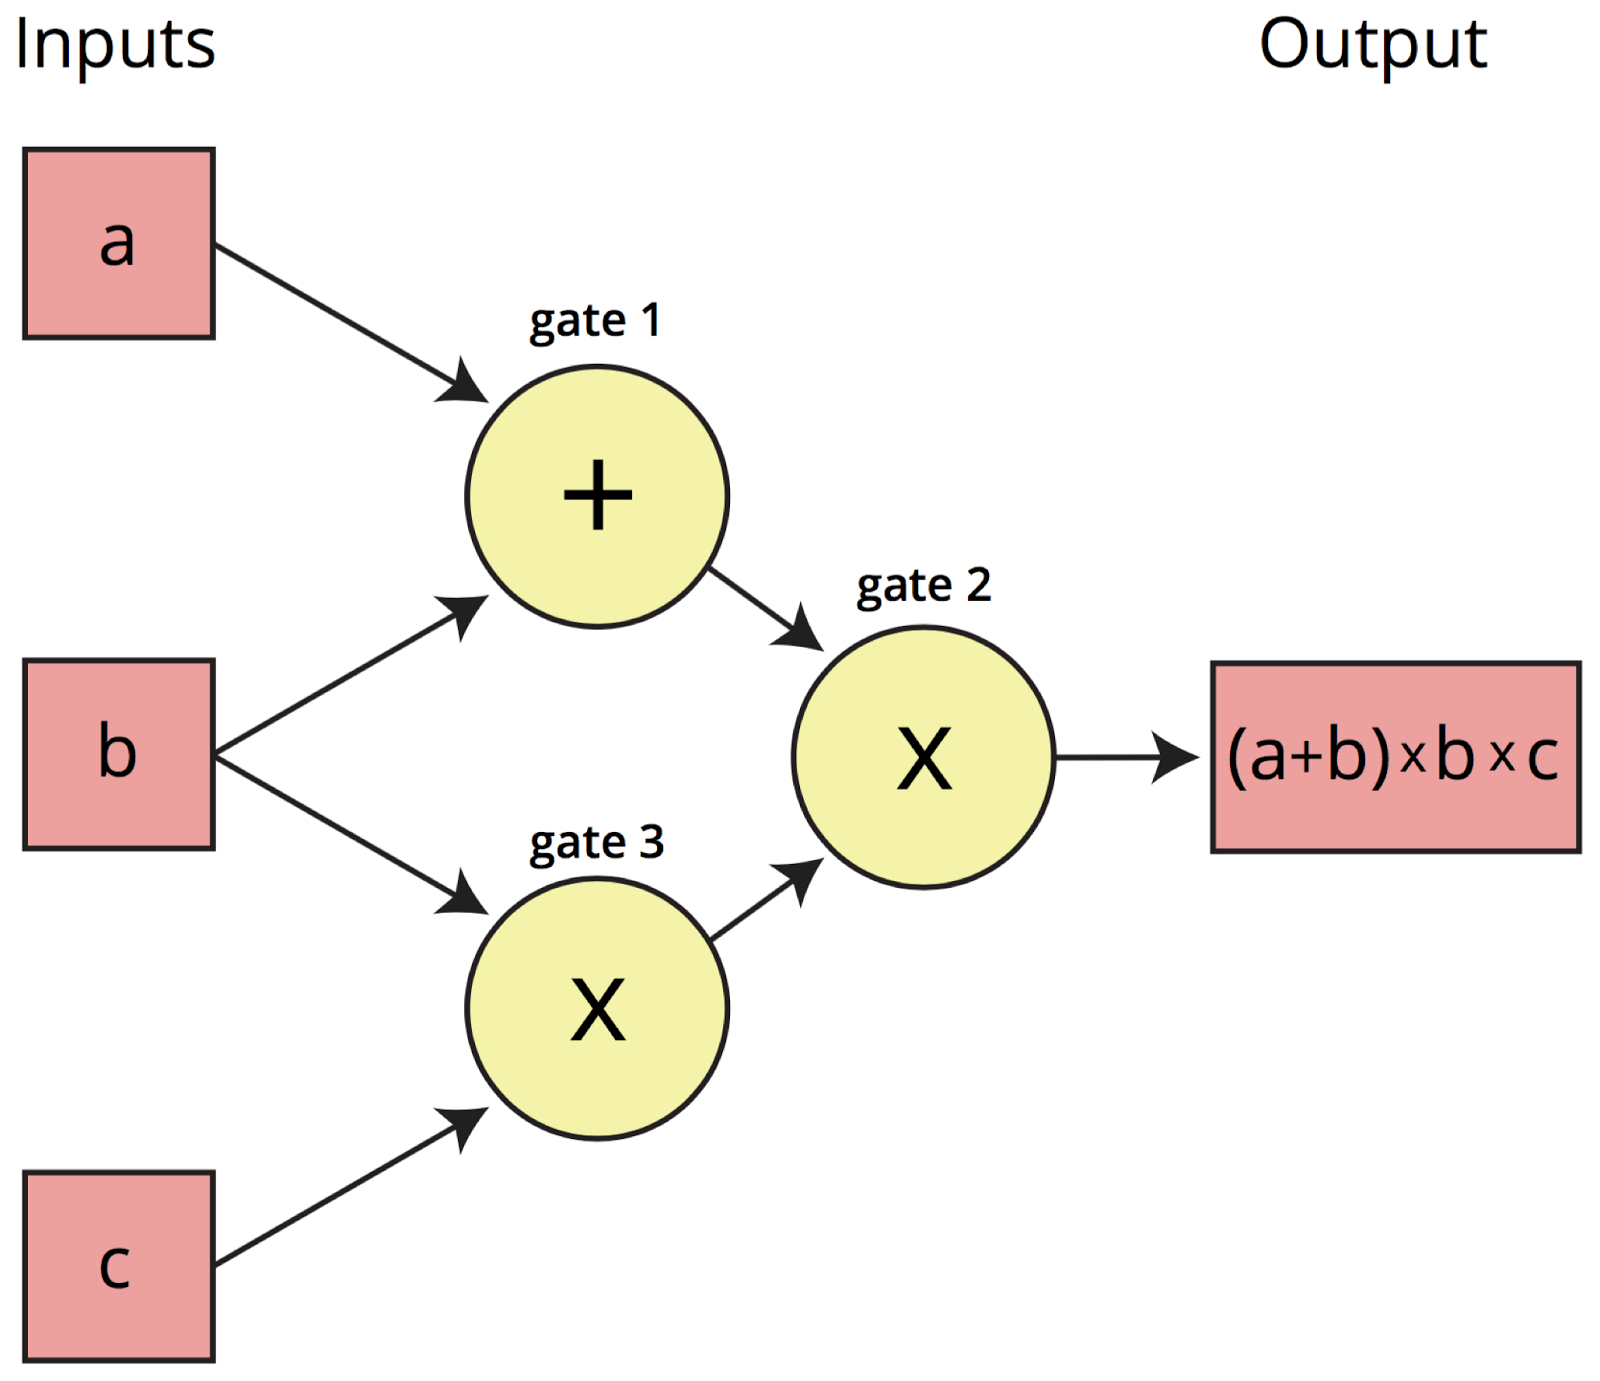
\includegraphics[width=.5\linewidth]{arithmetic-circuit.png}
	\caption {یک نمونه مدار محاسباتی}
	\label{fig:arithmetic}
\end{figure}

برای ساختن یک شاهد به این روش ابتدا محاسبات لازم را به یک مدار محاسباتی ریاضی تبدیل می‌کنیم به طوری که اثبات را به عنوان تعدادی شرط روی این مدار نشان دهیم، سپس به کمک یک
\lr{elliptic curve}
مقدار مدار را در چند نقطه‌ی تصادفی به عنوان اثبات ارائه می‌کنیم، با صادق بودن شرط‌ها در این نقاط شاهد را بررسی می‌کنیم. 
\\
برای انتخاب یکسان این نقاط تصادفی بین اثبات‌کننده و بررسی‌کننده نیاز به تعدادی نقطه‌ی توافق شده روی \lr{elliptic curve} داریم که باید در قبل از تولید اثبات انتخاب شده باشند. در این فاز آماده‌سازی تعدادی عدد تصادفی برای انتخاب این نقاط تولید می‌شوند که بعد از تولید نقاط باید بلافاصله پاک شوند. کسی که این اعداد (در واقع نقطه‌ی شروع روی منحنی) را داشته باشد می‌تواند شاهد‌های تقلبی ایجاد کند. برای تولید شاهد واقعی نیازی به دانستن این نقاط نیست و بنابراین بعد از فاز آماده‌سازی این اعداد باید پاک شوند. 
\subsubsection{ZK-STARK}
این روش مخفف
\lr{Zero-Knowledge Scalable Transparent ARguments of Knowledge}
است. مهم‌ترین وجه تمایز این روش در مقایسه با
\lr{ZK-SNARK}
 «شفافیت»
 \LTRfootnote{Transparency}
است، به این معنی که نیازی به فاز آماده‌سازی ندارد. عدم نیاز به آماده‌سازی و نداشتن زباله‌ی سمی (اطلاعاتی که باید پاک شوند تا امنیت سیستم تامین شود) این روش را برای کاربرد‌های حساس مناسب‌تر می‌کند اما در ازای این امنیت، حجم شاهد‌ها از چند صد بایت به چند صد هزار بایت تغییر می‌کند.
\par
ار مزیت‌های دیگر این روش استفاده نکردن از 
\lr{Elliptic curve}ها
است. نیاز‌های کم این روش باعث می‌شود که حتی با کامپیوتر‌های کوانتمی
\LTRfootnote{Quantum computers}
 راهی برای شکستن این اثبات‌ها وجود نداشته باشد.
\\
برای ساختن یک شاهد با این روش، برنامه‌ی مورد نظر را تبدیل یه یک چندچمله‌ای درجه بالا می‌کنند، سپس از مقدایر این چندجمله‌ای یک درخت مرکل ساخته می‌شود که مقدایر مختلف خروچی را نشان می‌دهد. سپس بررسی‌کننده چند شاخه از این درخت را به طور تصادفی انتخاب و بررسی می‌کند. برای غیرتعاملی کردن این اثبات می‌توان از هش ریشه‌ی درخت مرکل به عنوان ورودی یه تابع شبه‌تصادفی
\LTRfootnote{Pseudo random}
استفاده می‌شود که مشخص می‌کند خروجی کدام شاخه‌ها باید در شاهد بیاید. 





\cchapter{کارهای پیشین}

\cchapter{NotYetAdded}
\par
در این بخش به تعریف مفاهیم به کار برده شده در این تحقیق می پردازیم: 
\begin{itemize}
	\item 
	\textbf{بلاک‌چین}:
	بلاک‌چین ساختارداده ای است متشکل از بلوک های متوالی که هر یک هشی از بلوک قبلی‌اش را شامل می شود. در نتیجه برای ساختاری درست، باید با تغییر یک بلوک، تمام بلوک‌‌های بعد از آن را نیز تغییر داد. 
	\item
	\textbf{اثبات کار} \LTRfootnote{Proof of work}:
	روش اثبات کار بر اساس
	\lr{hashcash}
	\cite{hashcash}
	 -‌یک روش برای جلوگیری از حملات
	  \lr{DDoS}
	   طراحی شده است- ساخته شده است. روش کار 
	   \lr{hashcash}
	   بدین صورت است:
	   \\
	   برای این که یک ایمیل توسط سرور ارسال شود، همراه متن ایمیل کلاینت باید رشته‌ای ارسال کند تا اگر  هش 
	   \lr{SHA-1}
	   از آن گرفته شود ۲۰ بیت اول آن صفر شوند. به دلیلی تصادفی بودن هش رشته، باید با امتحان کردن رشته‌‌های مختلف به یک رشته‌ی مناسب رسید. زمان حل این مسئله‌ برای کامپیوتر‌های 
	   \lr{1 GHZ}
	   حدود یک ثانیه و یرای بررسی درست بودن آن هش تنها ۲ میکروثانیه است.
	   \\
	   زمان یک‌ ثانیه‌ای برای کاربر عادی که قصد ارسال یک ایمیل را دارد، قابل‌قبول است اما برای مهاجمی که قصد 
	   \lr{spam}
	   کردن توسط این سرویس را داشته باشد، یک ثانیه در ازای هر ایمیل هزینه‌ی زیادی خواهد بود.
	   \\
	   در بستر بیت‌کوین از این روش برای توافق بر بلوک‌های بعدی بلاک‌چین به صورت زیر استفاده می‌شود:
	   \\
	هر بلوک جدید شامل تعدادی تراکنش، برای ثبت در بلاک‌چین است تا توسط ماینترها به یک بلوک تبدیل شود. اما برای پذیرفته شدن این بلوک توسط دیگر ماینرها، باید در این بلاک یک nounce قرار گیرد به صورتی که هش بلاک از عددی که توسط پروتکل بیت‌کوین انتخاب می‌شود کمتر باشد. این شرط در طول زمان به صورت خودکار به روزرسانی می‌شود به طوری که در هر لحظه به صورت میانگین اضافه کردن یک بلوک ۱۰ دقیقه از کل شبکه زمان ببرد. از آنجایی که تنها راه یافتن همچین رشته‌ای بروت‌فورس
	\LTRfootnote{Bruteforce}
	 است، توان محاسباتی بالاتر احتمال یافتن بلوک بعدی را افزایش خواهد داد. 
	 \\
	
	
	\item 
	
\textbf{مسئله‌ی ژنرال‌های بیزنتین}: 
مسئله‌ی ژنرال‌های بیزنتین یا تحمل خطای بیزنتین مدلی از تحمل خطا در سیستم‌های توزیع شده است که در آن تعدادی ژنرال ارتش با هم به صورت پیام‌های یک به یک صحبت می‌کنند و در ساده‌ترین حالت در مورد حمله یا عقب‌نشینی در یک نبرد تصمیم می‌گیرند. اما تعدادی از آن‌ها خائن بوده و برای توافق غلط جمع تلاش می‌کنند (توافق درست توافقی است که اگر هیچ خائنی وجود نداشت به آن می‌رسیدند) و یا با جواب ندادن مانع تصمیم‌گیری آن‌ها شوند. در ساده‌ترین حالت و بدون استفاده از امضا‌های دیجیتال ثابت می‌شود که برای 3k + 1 ژنرال، با رای‌گیری می‌توان تا k خائن را تحمل کرد. 
	راه‌حل خلاقانه‌ی بیت‌کوین برای حل این مسئله استفاده از بلاک‌چین برای ذخیره‌ی اطلاعات و اثبات کار برای اضافه کردن بلوک به بلاک‌چین است. 
	\\
	برای نشان دادن نحوه‌ی حل این مسئله‌ مثالی را بررسی می‌کنیم؛ فرض می‌کنیم شخص A یک بیت‌کوین را به B منتقل کرده، این تراکنش در بلاک‌چین ثبت شده و در ازای آن کالایی دریافت کرده‌است، حال قصد دارد این تراکنش را از بلاک‌چین بیت‌کوین حذف کند تا بتواند آن را دوباره خرج کند. از آنجایی که نود‌های شبکه‌ی بیت‌کوین اگر ۲ زنجیره از بلوک‌ها دریافت کنند زنجیره‌ی بلند‌تر را قبول خواهند کرد باید قبل از این که کل شبکه یک بلوک  اضافه کند، دو بلوک سالم بسازد.
	\\
	احتمال موفقیت حمله‌ی A مساوی
	$(\frac{A's\ computational\ power}{Bitcoin\ network's\ computational\ power}) ^ 2 $
	است. اگر توان محاسباتی A از دیگر قسمت‌های شبکه کمتر باشد، این کسر عددی کوچک‌تر از 
	\lr{0.5}
	است. اگر این کار به موقع با موفقیت انجام نشود، سه بلوک عقب می‌افتد و توان فرمول بالا تبدیل به سه می‌شود و احتمال موفقیتش کمتر از پیش می‌شود. 
	\\
	این مسئله مسئله‌ی قمارباز
	\LTRfootnote{Gambler's Ruin}
	 نام دارد که نشان داده می‌شود در آن در طول زمان احتمال موفقت مهاجم به صورت نمایی کاهش پیدا می‌کند.
	
	\item 
	\textbf{انشعاب} \LTRfootnote{fork}:
	منظور از انشعاب در ارز‌های دیجیتال تبدیل یک بلاک‌چین به دو بلاک‌چین است. گاها برای ساخت ارز‌های جدید از بلاک‌چین موجود ارزهای دیگر مثل بیت‌کوین استفاده‌ می‌شود. این کار باعث شروع آسان‌تر و سریع‌تر بلاک‌چین می‌شود. در روال عادی کار بیت‌کوین نیز ممکن است انشعابی رخ دهد اما هر ماینری که متوجه انشعابی شود به صورت خود‌کار بلند‌ترین زنجیره را به عنوان زنجیره‌ی درست انتخاب می‌کند. هنگامی که یک انشعاب برای تولید بلاک‌چین جدید انجام گیرد و بلوک‌هایی قبلی آن همچنان درست حساب شوند این انشعاب را انشعاب نرم و مورد قبول سیستم‌ جدید نباشند انشعاب را انشعاب سخت می‌نامیم.
	\item 
	\textbf{ماین‌کردن}: 
	به عملیات ساختن بلوک‌های جدید بر بلاک‌چین با هدف پیدا کردن بلاک‌های درست و دریافت جایزه‌ی آن‌ها، ماین‌کردن می‌گوییم.
	\item 
	\textbf{ماینینگ‌ پول}:
	از آن‌ جای که ماین کردن برای یک نفر با توجه به کم بودن احتمال یافتن بلوک معتبر را زودتر از بقیه‌ی شبکه به صرفه نیست، ماینینگ‌پول‌ها شکل گرفته‌اند. با تقسیم کردن کار بین چندین ماشین شانس پیدا کردن بلوک معتبر بیشتر شده و جایزه‌ی ماین‌ کردن به نسبت توان محاسباتی بین شرکت‌کنندگان تقسیم می‌شود. برای بدست آوردن توان محاسباتی مصرف شده‌ی هر ماشین از تعداد بلوک‌هایی که هش آن‌ها به اندازه‌ی کافی برای درست بودن کوچک نیست ولی به جواب درست نزدیکند استفاده می‌شود.
	
	\item
	\textbf{قرارداد هوشمند}
	لفظ قرارداد‌های هوشمند اولین بار در سال ۱۹۹۳ توسط N.Szabo 
	\cite{SmartContract}
	به عنوان یک پروتکل تراکنش کامپیوتری که شروط یک قرارداد را اجرا می‌کند، مطرح شد. در اولین مثال معروف قرارداد‌های هوشمند یک وندینگ‌ ماشین
	\LTRfootnote{vending machine}
	 را مثال زد که در ازای سکه‌ی به طور اتوماتیک کالای مورد نظر را به مشتری می‌دهد، همچنین از آنجای که بدون سکه هرگز کالایی نمی‌دهد و صندوق، امنیت سکه ها را تا حدودی تأمین می کند، قرارداد مناسبی بین مشتری و تولیدکننده‌ی کالا محسوب می‌شود.
	هدف نهایی قراردادهای هوشمند کاهش نیاز به اعتماد کردن و افراد میانی در یک قرارداد است و با بسترهای ارز دیجیتال و راه‌حل‌های جدید مسئله‌ی ژنرال‌های بیزنتین بستر مناسبی برای ساخت قراردادهای هوشمند و توزیع‌شده بدون نیاز به اعتماد به شخص ثالث بوجود آمده است. 
	با وجود این که به کمک زبان اسکریپتینگ بیت‌کوین می‌توان مدل‌های مختلفی از قرارداد‌های هوشمند را تولید کرد، با اتریوم به کمک زبان برنامه‌نویسی turing-complete آن در تئوری می‌توان هر قرارداد هوشمند ممکن را تولید کرد. 
	
	
\end{itemize}

\cchapter{مروری بر پژوهش‌های مرتبط}
در این بخش به مروری بر کارهای انجام شده تاکنون می‌پردازیم. این مقالات را به سه دسته‌ی زیر تقسیم می‌کنیم.

\section{امنیت بلاک‌چین و ماین‌کردن}

در روش امنیتی بیت‌کوین که از طریق حل یک مسئله‌ی سخت محاسباتی ثابت بلاک‌های جدید به بلاک‌چین اضافه می‌شوند چند مسئله‌ی امنیتی رخ می‌دهد؛ نخست به دلیل این که عملیات ماین‌کردن نیازی به تمام بلاک‌چین ندارد و افراد می‌توانند کار را تقسیم کنند احتمال بوجود امدن یک ماینینگ پول که بیش از پنجاه‌ درصد توان محاسباتی را داشته باشد بالا می‌رود. بعضی پژوهش‌ها در این زمینه برای تولید مسائل مناسب برای اثبات کار، که در عین‌حال قابل تقسیم و موازی انجام شدن هم باشند، انجام شده است. 
\par
مورد‌ دیگر، بوجود آمدن سخت‌افزارهای مخصوص این مسئله‌ است که باعث می‌شود عملیات ماین کردن از یک عملیات توزیع‌شده که تمام افراد در آن شرکت می‌کنند یه عملیاتی که به سرمایه‌ی اولیه زیاد نیاز دارد، تبدیل شود. 
امنیت بیت‌کوین در گرو این موضوع است که به نفع تمامی ماینرهاست که پروتکل را رعایت کنند اما در این تحقیق
\cite{ResearchP}
 نشان داده شده که این گزاره همواره درست نیست و در بعضی شرایط به نفع ماینینگ‌پول‌هاست که از توان مصرفی خود در یک ماینینگ‌پول رقیب استفاده‌ کنند و اگر هش درست را برای رقیب پیدا کردند آن را اعلام نکنند
\cite{LongestChain}
. 
\\
تحقیق دیگر 
\cite{Majority}
نشان داد در شرایطی برای به نفع ماینینگ‌پول‌هاست که اگر هش درست را پیدا کردند به دیگران اعلام نکنند تا برای بلوک بعدی به دلیل زودتر شروع کردن شانس بیشتری داشته باشند. 
\par
با توجه به این شرایط و همچنین هزینه‌ی محاسباتی بالایی که ماین‌کردن در شرایط فعلی بیت‌کوین و بسیاری از ارزهای دیجیتال دیگر دارد تحقیقات بسیاری برای پیدا کردن روش‌های دیگر به جای استفاده از اثبات کار برای اضافه کردن بلوک به بلاک‌چین شده که در ادامه به تعدادی از آن‌ها اشاره می‌کنیم:
\\
\begin{itemize}
	\item \textbf{اثبات سهم}
	\LTRfootnote{proof of stake}
	:
	به این صورت است که هر ماین‌کننده‌ای که سهم بیشتری در سکه‌های بستر داشته باشد، شانس بیشتری برای ساختن بلوک بعدی دارد. ایده‌ی کلی این روش این است که در صورت بروز مشکلی برای بستر، این افراد بیشترین ضرر را خواهند کرد. 
	\item \textbf{اثبات سن سکه}\LTRfootnote{proof of coin-age}:
	یک روش ارائه شده توسظ 
	\lr{Peercoin}
	است که در آن برای ماین کردن به مقدار سکه‌ی قدیمی (عمر سکه مدت زمانی که در یک حساب ساکن مانده باشد تعریف می‌شود) هر ماین‌کننده توجه می‌شود.
	\item \textbf{اثبات سپرده}\LTRfootnote{proof of deposit}:
	در این روش برای ساخت بلوک‌ جدید باید مقداری سکه توسط ماین‌کننده در یک حساب برای مدت زمانی قفل شوند.
	\item \textbf{اثبات سوزاندن}\LTRfootnote{proof of burn}:
	در این روش برای ساخت بلوک‌ باید مقداری سکه را به حسابی غیرقابل دسترس (مثلا حسابی با کلید عمومی تماما صفر) منتقل کرد.
	\item \textbf{اثبات فعالیت}\LTRfootnote{proof of activity}:
	در این روش تعدادی کاربر در هر مرحله به صورت تصادفی  برای اضافه‌کردن بلوک انتخاب می‌شوند و باید در مدت زمانی محدود با یک پیغام امضا شده به آن پاسخ دهند. 
	\item \textbf{\lr{Stellar Consensus Protocol}}\cite{scp}:
	در این روش با بوجود آمدن طبیعی کاربرهای قابل اعتماد و ساخت لایه‌هایی از اعتماد که بی‌شباهت به لایه‌های 
	\lr{ISP}
	نیست، برای انتخاب بلوک بعدی تصمیم می‌گیرند. همچنین هر کاربر خود انتخاب می‌کند که چه افرادی در مورد درستی تراکنش او تصمیم بگیرند.
\end{itemize}

\section{امنیت قرارداد‌های اتریوم}

بدیهی است که با بوجود آمدن ارزهای دیجیتال مانند بیت‌کوین و تراکنش‌های نیمه‌ناشناس در آن‌ها بستری مناسبی برای تراکنش‌های غیرقانونی و مجرمانه بوجود آمد، به کمک بستر اسکرپیتینگ بیت‌کوین و در ادامه بستر کامل قرارداد‌های هوشمند مسئله‌ی قرارداد‌های مجرمانه به طور جدی‌تری مسئله خواهد شد. در تحقیق‌های 
\cite{gyges} \cite{smart}
به بررسی دقیق‌تر این کاربردها پرداخته شده است. برای مثال قراردادهایی برای لو دادن اسناد محرمانه و یا حتی دزدین کلید‌های رمزنگاری از جمله کاربرد‌های ممکن این قراردادها هستند. 
\\
همچنین atezi
\cite{surveyAtt}
 به بررسی مشکلات امنیتی معمول قراردادهای در بستر اتریوم و تله‌ی معمول این زبان برنامه‌نویسی و روش‌های تصحیح آن‌ها پرداخت. از اشتباهاتی که وی در تحقیق خود به آن‌ها پرداخته می‌توان به نحوه‌ی نوشتن قراردادی که در سال ۲۰۱۶ باعث انشعاب بلاک‌چین اتریوم شد اشاره کرد. 
 
\section{حریم خصوصی}
از کارهای دیگر بر روی امنیت تراکنش‌ها می‌توان به تلاش‌هایی برای تبدیل کردن این بستر‌ها از بسترهای تراکنش نیمه‌ناشناس به تراکنش‌های ناشناس اشاره کرد. کارهایی مانند 
\lr{zerocash} 
\cite{zerocash}
و بستر 
\lr{HAWK}
\cite{hawk}
و یا 
\lr{E. Heilman}
در مقاله‌ی 
\cite{blind}
به بررسی روش‌های تولید تراکنش‌های کاملا ناشناس بر روی بستر‌های موجود یا خارج از آن‌ها پرداخته‌اند. 
\cchapter{طرح مسئله‌}

با بوجود آمدن سازمان‌های خودکار توزیع‌شده در بستر اتریوم تلاش‌های بسیاری برای ساخت سازمان‌هایی برای کاربردهایی که در ساختار فعلی جامعه‌ احتیاج به اعتماد به یک سازمان مرکزی دارند در بستر بلاک‌چین شده است .
\\
یکی از این کاربردها سیستم‌های رای‌گیری هستند. در شرایط فعلی برای راه انداختن یک سیستم رای‌گیری سیستم‌های خودکاری وجود دارند که استفاده‌ از آن‌ها نیازمند اعتماد به نگه‌دارندگان آن سیستم‌ها (که در بسیاری از کاربردها دولت‌ها این نقش را به عهده دارند) و همچنین امنیت‌ این سیستم‌هاست. 
\\
یک تحقیق معروف از دانشگاه‌ \lr{NYU} در سال ۲۰۱۵ 
\LTRfootnote{https://www.brennancenter.org/publication/americas-voting-machines-risk}
توضیح داد که ماشین‌های رای‌گیری الکترونیکی که در ۴۳ ایالت آمریکا استفاده می‌شوند در سال ۲۰۱۶ به دهمین سال استفاده شدن می‌رسند. ساختار و نرم‌افزار قدیمی این دستگاه‌ها باعت می‌شود که احتمال هک شدن آن‌ به شدت بالا برود. 
\\
در سال ۲۰۱۶  اوکراین و ایالات متحده‌ی آمریکا قراردادی برای ساخت یک سیستم‌ رای‌گیری بر روی بستر اتریوم امضا کردند
\LTRfootnote{http://www.coinfox.info/news/4794-ukraine-to-introduce-etherium-based-e-voting}
. این پتانسیل تکنولوژی بلاک‌چین در زمینه‌ی رای‌گیری باعث تولید چند نمونه 
\cite{rosgood}
از سیستم‌های رای‌گیری بر بستر بلاک‌چین نیز شده که از آن‌ها می‌توان به 
\lr{VoteBook}
\cite{votebook}
توسط شرکت 
\lr{Kaspersky}
که یک شرکت پیشرو دز زمینه‌ی امنیت است اشاره کرد.

فلسفه‌ی ساخت این سیستم به صورتی است که تلاش می‌کند برای کاربرانی که از سیستم‌هایی رای‌گیری فعلی استفاده می‌کنند کمترین تغییر در رفتار نیاز باشد. 
\\
از مثال‌های دیگر سیستم‌های رای‌گیری مبتنی بر بلاک‌چین می‌توان به استارت‌آپ 
\lr{Follow My Vote}
اشاره کرد. نجوه‌ی کار این سیستم با سیستم 
\lr{VoteBook}
تفاوت اساسی دارد و برای رای‌دادن احتیاج دارد که نرم‌‌افزاری برای رای‌دادن به روی کامپیتور و یا تلفن‌همراه کاربران نصب شود. 
\\
و در نهایت یکی از موفق‌ترین سیستم‌های رای‌گیری مبتنی بر بلاک‌چین موجود در حال حاضر 
\lr{VoteWatcher}
ساخته شده توسط یک شاخه از شرکت 
\lr{blockchain Technologies Corporation}
است که یک شرکت بزرگ برای ارائه‌ی سرویس‌های مبتنی بر بلاک‌چین است. طبق وب‌سایت این محصول تاکنون بیش از صدهزار رای در بیشتر از ۲۰ رای‌گیری مختلف توسط این سیستم‌ شمارش شده‌است. 
\\
مدل اسفاده‌ی 
\lr{VoteWatcher}
به سیستم‌ 
\lr{VoteBook}
بسیار شبیه است و تفاوت رفتاری زیادی با مدل‌های رای‌گیری الکترونیکی فعلی برای کاربران ندارد. 
\\
یک نکته‌ی مهم در مورد همه‌ی این نمونه‌ها این است که در آن‌ها استفاده‌ای از بلاک‌چین‌های عمومی نمی‌شود و با استفاده از بلاک‌چین‌های اختصاصی کار می‌کنند. در حالت کلی این یک نکته‌ی منفی ولی بسته‌ به کاربرد می‌تواند استفاده‌ از یک بلاک‌چین عمومی به شفافیت سیستم کمک کند.
\\
یک مسئله‌ی دیگر که با وجود امنیت بالای این سیستم‌ها هنوز حل نشده و جای کار دارد سیستم‌های رای‌گیری برای شرایطی که امنیت رای‌دهندگان را نمی‌شود به خوبی تامین کرد است. با وجودی که اکثر سیستم‌های فعلی از قابلیت انتخاب این که رای این رای‌دهنده شمارش نشود پشنیبانی می‌کنند، سیستم پیگیری رای که برای امنیت و اطمینان ییشتر به سیستم اضافه شده می‌تواند حریم خصوصی کاربران را زیر سوال ببرد.
\\ 
\lr{R. Sarres de Almeida}
در یک بلاگ پست به این مسئله در برزیل و مشکلاتی که این سیستم به وضعیت خرید و فروش و یا تهدید برای رای دادن به یک کاندیدای خاص بوجود می‌آورد پرداخت. در شرایطی که فردی که رشوه داده می‌تواند 
\lr{Ballot ID}
کسی که رای داده را از او گرفته و نتیجه‌ی رای او را چک کند، خطر خرید و فروش و بخصوص استفاده از خشونت برای جمع‌کردن رای دوچندان می‌شود. 
\\
با توجه به این خلا موجود در پیاده‌سازی‌های موجود در این زمینه، هدف این پژوهش طراحی یک سیستم رای‌گیری دیجیتال مبتنی بر بلاک‌چین است که در آن بتوان شمارش هر رای را بررسی کرد ولی امکان وصل کردن به رای داده شده به هیچ وجه ممکن نباشد. 






